\section*{Functionel Description Report}
\tableofcontents
\newpage

\section{Abstract}

\section{Introduction}
The security of wireless networks has become increasingly important as more and more devices are connected to the internet. However, even with the use of encryption and other security measures, wireless networks are still vulnerable to attacks from hackers. One such attack is the creation of a rogue Access Point (AP), which can be used to intercept and manipulate network traffic.

In this project, we will explore the creation of a rogue AP for the purpose of sniffing network traffic and deauthenticating clients on the network. The rogue AP will be designed to mimic a legitimate AP, allowing it to attract clients and capture their traffic. Additionally, we will implement deauthentication attacks to force clients to disconnect from the legitimate AP and connect to our rogue AP, giving us access to their network traffic.

Furthermore, we will also study the 4-way handshake process used in wireless network authentication. We will use this knowledge to perform password cracking attacks on captured network traffic. By analyzing the encrypted handshake packets, we will attempt to crack the pre-shared key (PSK) used for network authentication.

The password cracking process will involve using various tools and techniques, such as dictionary attacks and brute-force attacks, to crack the PSK. We will explore the effectiveness of these methods and discuss countermeasures that can be employed to strengthen the security of wireless networks against such attacks.

Through this project, we aim to highlight the vulnerabilities of wireless networks and demonstrate the importance of securing them. It is important to note that this project is for educational purposes only and should not be used for malicious activities. Overall, this project will provide a comprehensive understanding of the vulnerabilities of wireless networks and the importance of implementing strong security measures. It will also equip participants with the knowledge and skills required to protect their own networks from similar attacks.




\section{Functionality}
Our project is made up of these functionalities:
\begin{enumerate}
    \item Scan local networks (Maybe even identify)
    \item Become an AP
    \item Deauthentication attacks
    \item 4-way handshake
    \item Password cracking
\end{enumerate}

 
These functionalities aim to be the core of the product that will be created. The first functionality, Scanning for local networks, is the most important one as that is the basis of all other functionalities. 
Becoming an AP is the function that allows the product to allow Wi-Fi devices to connect to the product. It acts as a central transmitter and receiver of the wireless radio signals. 

A deauthentication attack is a type of denial-of-service attack that targets communication between a user and a Wi-Fi wireless access point. It exploits a feature of IEEE 802.11 wireless networks that allows devices to disconnect from a network by sending deauthentication frames.

A deauthentication frame is a message that tells a device to stop using the network. It can be sent by either the access point or the device itself. Normally, it is used for legitimate purposes, such as ending a connection or switching to another network.

However, an attacker can also send deauthentication frames to any device associated with an access point, using a tool such as Aircrack-ng3. This causes the device to lose its connection and try to reconnect, which consumes bandwidth and resources. If done repeatedly or to multiple devices, this can disrupt or disable the network entirely.

A 4-way handshake is a process that occurs when a device wants to join a Wi-Fi network that uses WPA or WPA2 encryption. It involves exchanging four messages between the device and the access point to generate encryption keys that can be used to secure data transmission. The product should be able to this by doing the four steps which are as follows.
\begin{itemize}
    \item The access point sends a nonce to the device
    \item The device uses the nonce, its own nonce, and a pre-shared key (PSK) to generate a pairwise transient key (PTK) and then the device sends its nonce and a message integrity code to the access point
    \item The access point uses both nonces and the PSK to generate its own PTK and verify the MIC and  sends another MIC and a group temporal key (GTK) to the device
    \item The device verifies the MIC and sends another MIC to confirm
\end{itemize}
By implementing the four steps the product should then be able to connect to a broad range of devices and thereby become an AP.

The last point is password cracking. The product should be able to crack basic passwords in the WEP algorithm as that is one of the most basic security algorithms. It is and outdated and insecure algorithm and the product can use some of the multitude of tools available to crack it, like Aircrack-ng's PTW and FMS or WEPcrack. Alternatively we can create our own algorithm for cracking WEP if time permits.

We are going to write in python using scapy to implement the functions. We are also using Debian Linux to allow monitor mode on the wireless network cards. Hopefully we can use a raspberry pi later in the project when all the code has been written and is easily able to be placed onto the raspberry pi. 
If we are not able to use a raspberry pi the product will use a Realtek DWA 131-E1 dongle that creates a wlan adapter and allows monitor mode. This has the consequence that linux is required and that everything runs through a python program on a computer.
The positive side of using linux is that we can implement the program on many types of systems as we use a VM to create the product and makes conversion to a raspberry pi easier. The negative side is that we have to use a VM which can create problems with drivers and performance. 

\section{Blocks and sub-blocks}



\section{Theory}
The main theory behind this project is the 802.11 standard.
The 802.11 standard, is a set of wireless network protocols developed by the Institute of Electrical and Electronics Engineers (IEEE). The first version of the standard, 802.11, was released in 1997, and since then, several revisions and amendments have been made to improve the technology and increase its capabilities.

The 802.11 standard uses radio waves to transmit data between devices within a local area network (LAN) without the need for cables or wires. This makes it a popular choice for connecting devices to the internet, especially in homes, offices, and public places such as cafes, airports, and hotels.

The original 802.11 standard operated in the 2.4 GHz frequency band and provided a maximum data rate of 2 Mbps. However, subsequent versions, including 802.11b, 802.11a, 802.11g, and 802.11n, increased the data rate and expanded the frequency band to include 5 GHz.

802.11b was the first widely adopted WiFi standard, released in 1999, and provided a maximum data rate of 11 Mbps. It operates in the 2.4 GHz frequency band and is backward compatible with the original 802.11 standard.

802.11a, released in 1999, operates in the 5 GHz frequency band and provides a maximum data rate of 54 Mbps. However, due to its shorter range compared to 802.11b, it was not as widely adopted.

802.11g, released in 2003, operates in the 2.4 GHz frequency band and provides a maximum data rate of 54 Mbps. It is backward compatible with 802.11b and became the dominant WiFi standard for several years due to its high data rate and compatibility with older devices.

802.11n, released in 2009, improved the data rate further, with a maximum of 600 Mbps. It uses both the 2.4 GHz and 5 GHz frequency bands and introduced multiple input multiple output (MIMO) technology, which allows for multiple antennas to transmit and receive data simultaneously. This improves the signal strength and range of the network.


\begin{figure}[!htbp]
    \centering
    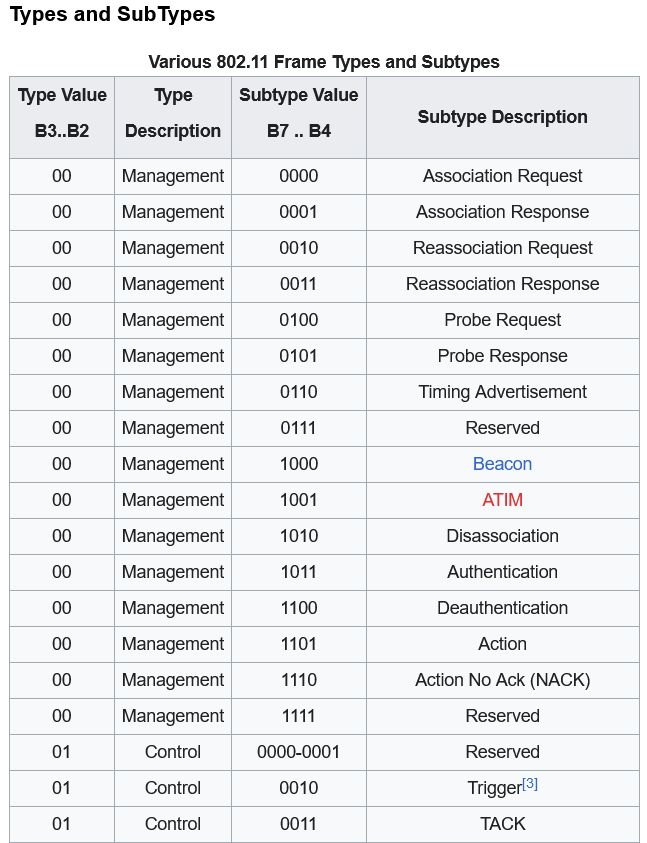
\includegraphics[width=0.6\textwidth]{Latex-Files/Billeder/WIFI_Types.png}
    \caption{WiFi typer og subtyper}
    \label{Wifi Types}
\end{figure}

802.11 also describes frames, which is the what data is made up of. Frames have specific purposes like an association request, probe request or beacon. There are parts of frames that are always present, these are parts of the frame control and the FCS, which is the error correcting part of the frame. The parts of frame control that are present are protocol version, type and subtype. Figure \ref{Wifi Types} shows some of the types and subtypes of different frames. 

\section{Conclusion}

\newpage
\section{Time Plan}
\begin{figure}[!htbp]
    \centering
    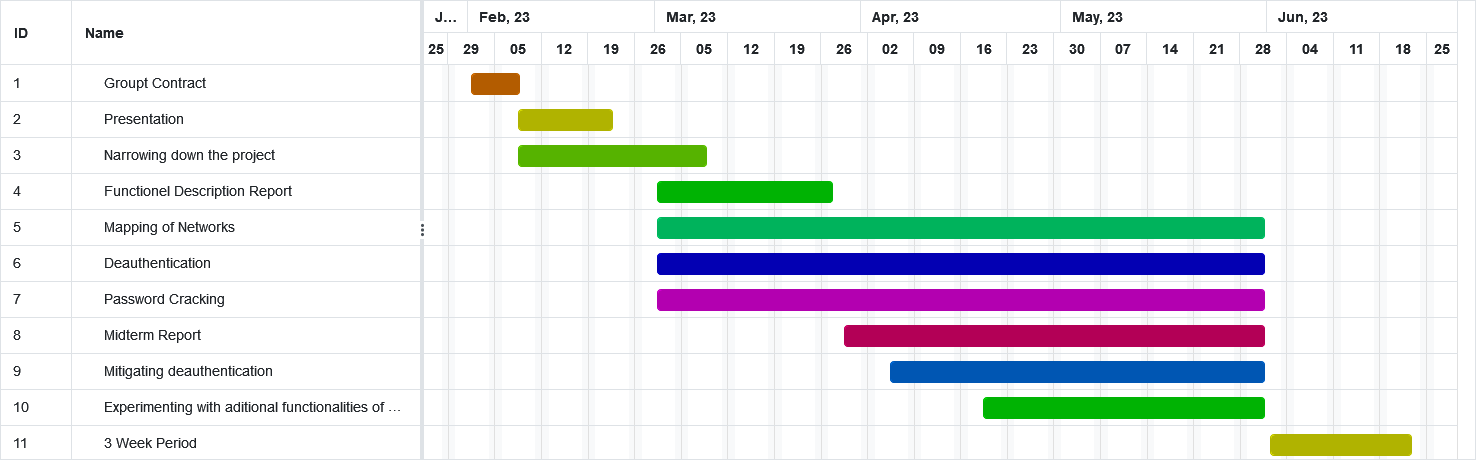
\includegraphics[width=1\textwidth]{Latex-Files/Billeder/Timeplan.png}
    \caption{Timeplan}
\end{figure}
